\chapter{Arhitektura i dizajn sustava}

		Web aplikacija "Čuvari pasa" izvedena je u arhitekturi klijent-poslužitelj. Klijenti (korisnici) šalju zahtjeve za nekom uslugom poslužitelju (web aplikaciji). Poslužitelj odgovara sa traženom uslugom ili statusom pogreške (HTTP status 404). Glavni cilj ove arhitekture je centralizirani sustav koji dijeli informacije i usluge.
		Nadalje se arhitektura može podijeliti na web poslužitelj, web preglednik i bazu podataka.\\
		\newline
		\textbf{Web poslužitelj} je zapravo funkcionalnost web aplikacije. On komunicira s klijentom preko web preglednika. Primarna uloga mu je "nabavljanje" HTTP zahtjeva i slanje HTTP odgovora. Ovisno o zahtjevu, web poslužitelj komunicira i s bazom podataka u kojoj se nalaze potrebni podaci. 
		\newline
		\textbf{Web preglednik} je softver koji služi kao sučelje između poslužitelja i klijenta i web dokumente klijentu. Njegova primarna uloga je slanje HTTP zahtjeva i primanje HTTP odgovora. Web preglednici prevode kod koji dobivaju u HTTP odgovoru te ga zatim prikazuju.
		\newline
		\textbf{Baza podataka} (podatkovni sloj) koristi se za sigurno spremanje podataka. Povezana je s web aplikacijom koja joj šalje upite za potrebnim podacima. Baza podataka je dalje opisana u poglavlju 4.1 Baza podataka.
		\newline
		\newline
		Web aplikacija koristi arhitekturu MVC (Model-View-Controller). \textbf{Model} predstavlja dinamičke strukture podataka. U njemu se izravno upravlja podacima.
		\textbf{View} predstavlja prikaz podataka, a \textbf{Controller} prima zahtjeve i prosljeđuje ih gdje su dalje potrebni. MVC je implementiran u našu web aplikaciju tako da su Model i Controller komponente sadržane u back-end dijelu, a view u front-end dijelu. \textbf{Front-end} (prezentacijski sloj) je dio aplikacije zaslužan za grafičko korisničko sučelje dok se \textbf{back-end} (poslovni sloj) može poistovjetiti sa web poslužiteljem. U njemu se opisuju funkcionalnosti web aplikacije odnosno on upravlja web aplikacijom.\\
		Backend je osim na model (repository) i controller komponente podijeljen i na service komponentu. U njoj se nalazi implementacija poslovne logike.
		\newline
		Front-end smo odlučili raditi u programskom jeziku JavaScript koristeći radni okvir React, a back-end u programskom jeziku Java s radnoim okvirom Spring Boot. Razvojna okruženja u kojima radimo su Visual Studio Code i IntelliJ.
		
		\begin{figure}[htb]
			\centering
			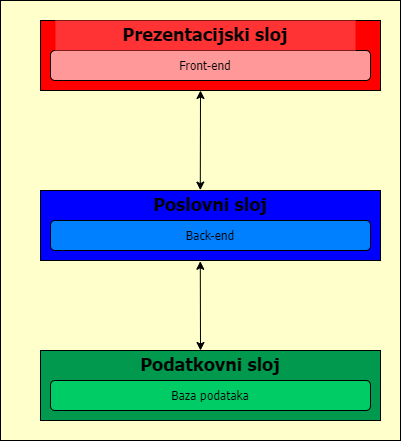
\includegraphics[width=10cm]{slike/arhitektura-diagram}
			\caption{Dijagram arhitekture} 
			\label{fig:arhitektura-dijagram}
		\end{figure}
		

	
		

		
		\eject
				
		\section{Baza podataka}
			
			Sustav koristi relacijsku bazu podataka koja će biti implementirana u PostgreSQLu. Relacijsku bazu podataka koristimo radi lakšeg oblikovanja sustava kao stvarnog svijeta, a PostgresSQL jer smo najbolje upoznati s njim. U njemu se entiteti modeliraju kao tablice koje imaju vlastito ime i skup atributa.\\
			Baza podataka nam je potrebna zbog njezine sigurnosti podataka, ali i brzog dohvata, pohrane i izmijene podataka koje sustav koristi za daljnje akcije.
			Baza podataka ovog sustava korisit sjedeće entitete:
			\begin{packed_item}
				\item Role
				\item App User
				\item Breed
				\item Owner
				\item Guardian
				\item Dog
				\item Request Dog
				\item Request Guardian
				\item Request Guardians Dog
				\item Activity
				\item Request Activity
				\item Agreed request
				
			\end{packed_item}
			
		
			\subsection{Opis tablica}
			
			
			\textbf{Role} je entitet koji sadržava sve važne informacije o rolama aplikacije. Povezan je vezom One-To-Many s tablicom App User preko atributa userId tablice App User. Sadrži atribute: roleId i name.
			
			
			
			
			\begin{longtblr}[
				label=none,
				entry=none
				]{
					width = \textwidth,
					colspec={|X[6,l]|X[6, l]|X[20, l]|}, 
					rowhead = 1,
				} %definicija širine tablice, širine stupaca, poravnanje i broja redaka naslova tablice
				\hline \multicolumn{3}{|c|}{\textbf{Role}}	 \\ \hline[3pt]
				\SetCell{LightGreen}roleId	& INT &  Jedinstven identifikator uloge korisnika 	\\ \hline
				name & VARCHAR &  Ime role u sustavu \\ \hline
			 
			\end{longtblr}
			
			\textbf{App User} je entitet koji sadrži sve važne informacije o korisniku aplikacije. Povezan je vezom Many-To-One s tablicom Role preko vlastitog atributa userId. Tablica Owner je specifikacija ove tablice pa je povezana s njom vezom Many-To-One preko userIda. Isto vrijedi i za tablicu Guardian. S tablicom Dog ima vezu Many-To-One koja je isto povezana preko atributa userId. Isto vrijedi za tablice Request Dog, Request Guardian i Agreed Request. Vlastiti atributi su: userId, roleId, username, firstName, lastName, password, ratingSum, ratingCount i email.

				
				
				
				\begin{longtblr}[
					label=none,
					entry=none
					]{
						width = \textwidth,
						colspec={|X[6,l]|X[6, l]|X[20, l]|}, 
						rowhead = 1,
					} %definicija širine tablice, širine stupaca, poravnanje i broja redaka naslova tablice
					\hline \multicolumn{3}{|c|}{\textbf{App User}}	 \\ \hline[3pt]
					\SetCell{LightGreen}userId & INT	&  	Jedinstveni identifikator korisnika\\ \hline
					\SetCell{LightBlue}roleId	& INT &  Jedinstven identifikator uloge korisnika (Role.roleId) \\ \hline
					username & VARCHAR &  Korisničko ime u sustavu \\ \hline 
					firstName & VARCHAR	&  	Ime korisnika	\\ \hline
					lastName & VARCHAR	&  	Prezime korisnika	\\ \hline
					password & VARCHAR	&  	Hash lozinke korisnika	\\ \hline 
					ratingSum & INT	&  	Zbroj svih ocjena	\\ \hline 
					ratingCount & VARCHAR	&  	Zbroj svih ocjenjivanja	\\ \hline 
					email & VARCHAR	&  	Email pošta korisnika	\\ \hline 
				\end{longtblr}
			
			
			\textbf{Breed} je entitet koji razlikuje sve pasmine u sustavu. Povezan je vezom Many-To-One s tablicom Dog preko atributa breedId. Isto vrijedi i za tablicu Request Dog. Sadrži atribute: breedId i name.
		
		\begin{longtblr}[
				label=none,
				entry=none
				]{
					width = \textwidth,
					colspec={|X[6,l]|X[6, l]|X[20, l]|}, 
					rowhead = 1,
				} %definicija širine tablice, širine stupaca, poravnanje i broja redaka naslova tablice
				\hline \multicolumn{3}{|c|}{\textbf{Breed}}	 \\ \hline[3pt]
				\SetCell{LightGreen}breedId & INT	&  	Jedinstveni identifikator pasmine\\ \hline
				name	& VARCHAR &  Naziv pasmine	\\ \hline 
				
			\end{longtblr}
		
				\textbf{Owner} je entitet koji sadrži sve važne informacije o vlasnicima pasa. On je specifikacija entiteta appUser pa sadrži njegove atribute. userId mu je primarni ključ kao i strani ključ koji referencira na atribut userId u entitetu App User. Povezan je vezom Many-To-One s tablicom Dog preko userIda, a isto vrijedi i s tablicom Request Guardian.
			
			\begin{longtblr}[
				label=none,
				entry=none
				]{
					width = \textwidth,
					colspec={|X[6,l]|X[6, l]|X[20, l]|}, 
					rowhead = 1,
				} %definicija širine tablice, širine stupaca, poravnanje i broja redaka naslova tablice
				\hline \multicolumn{3}{|c|}{\textbf{Owner}}	 \\ \hline[3pt]
				\SetCell{LightBlue}userId & INT	&  	Jedinstveni identifikator vlasnika pasa, (App User.userId)\\ \hline
				
			\end{longtblr}
		
				\textbf{Guardian} je entitet koji sadrži sve važne informacije o čuvarima pasa. On je specifikacija entiteta appUser pa sadrži njegove atribute. userId mu je primarni ključ kao i strani ključ koji referencira na atribut userId u entitetu App User. Povezan je vezom Many-To-One s tablicom Request Guardian preko atributa userId. Još ima vlastite atribute: hasExperience i hasDog.
			
			\begin{longtblr}[
				label=none,
				entry=none
				]{
					width = \textwidth,
					colspec={|X[6,l]|X[6, l]|X[20, l]|}, 
					rowhead = 1,
				} %definicija širine tablice, širine stupaca, poravnanje i broja redaka naslova tablice
				\hline \multicolumn{3}{|c|}{\textbf{Guardian}}	 \\ \hline[3pt]
				\SetCell{LightBlue}userId & INT	&  	Jedinstveni identifikator čuvara pasa, (App User.userId)\\ \hline
				hasExperience	& BOOLEAN &  Ima li čuvar iskustvo	\\ \hline 
				hasDog	& BOOLEAN &  Ima li čuvar vlastitog pasa	\\ \hline 
				
			\end{longtblr}
		
			\textbf{Dog} je entitet koji sadrži sve važne informacije o psima vlasnika. Povezan je vezom One-to-Many s tablicom Owner preko userIda i s tablicom Breed preko breedIda. Vezom Many-To-One povezan je s tablicom Request Guardians Dog preko atributa dogId. Još ima atribute: name, dateOfBirth, photo, ratingSum i ratingCount.
			\begin{longtblr}[
				label=none,
				entry=none
				]{
					width = \textwidth,
					colspec={|X[6,l]|X[6, l]|X[20, l]|}, 
					rowhead = 1,
				} %definicija širine tablice, širine stupaca, poravnanje i broja redaka naslova tablice
				\hline \multicolumn{3}{|c|}{\textbf{Dog}}	 \\ \hline[3pt]
				\SetCell{LightGreen}dogId & INT	&  	Jedinstveni identifikator pasa\\ \hline
				name	& VARCHAR &  Ima li čuvar iskustvo	\\ \hline 
				dateOfBirth	& DATE &  Datum rođenja psa	\\ \hline 
				photo	& VARCHAR &  Slika pasa	\\ \hline
				ratingSum	& INT &  Suma svih ocjena	\\ \hline
				ratingCount	& VARCHAR &  Suma svih ocjenjivanja	\\ \hline
				\SetCell{LightBlue}userId	& INT &  jedinstveni identifikator vlasnika pasa, (App User.userId)	\\ \hline
				\SetCell{LightBlue}breedId	& INT &  jedinstveni identifikator pasmine, (Breed.breedId)	\\ \hline
				
			\end{longtblr}

			\textbf{Request Dog} je entitet koji sadrži sve važne informacije o zahtjevima koje vlasnici pasa šalju. Povezan je vezom One-To-Many s tablicom Breed preko breedIda i s tablicom Guardian preko atributa userId. Vezom Many-To-One je povezan s tablicom Agreed Request preko atributa requestDogId. Još ima atribute: dogAge, dogTimeBegin, dogTimeEnd, isFlexible, location, numberOfDos, isPusblished i isReviewed.
			\begin{longtblr}[
				label=none,
				entry=none
				]{
					width = \textwidth,
					colspec={|X[6,l]|X[6, l]|X[20, l]|}, 
					rowhead = 1,
				} %definicija širine tablice, širine stupaca, poravnanje i broja redaka naslova tablice
				\hline \multicolumn{3}{|c|}{\textbf{Request Dog}}	 \\ \hline[3pt]
				\SetCell{LightGreen}requestDogId & INT	&  	Jedinstveni identifikator zahtjeva slanog od vlasnika\\ \hline
				dogAge	& INT &  Dob pasa	\\ \hline 
				dogTimeBegin	& TIMESTAMP  &  Početak čuvanja pasa	\\ \hline 
				dogTimeEnd	& TIMESTAMP  &  Završetak čuvanja pasa	\\ \hline
				isFlexible	& BOOLEAN &  Je li vrijeme čuvanja fleksibilno	\\ \hline
				location	& VARCHAR &  Lokacija stanovanja vlasnika	\\ \hline
				numberOfDos	& INT &  Broj pasa	\\ \hline
				isPusblished	& BOOLEAN &  Je li zahtjev oglašen	\\ \hline
				isReviewed	& BOOLEAN &  Je li pas i njegov vlasnik ocjenjivan	\\ \hline
				\SetCell{LightBlue}userId	& INT &  jedinstveni identifikator čuvara pasa, (Guardian.userId)	\\ \hline
				\SetCell{LightBlue}breedId	& INT &  jedinstveni identifikator pasmine, (Breed.breedId)	\\ \hline
				
			\end{longtblr}
		
			\textbf{Request Guardian} je entitet koji sadrži sve važne informacije o oglasima koje čuvari pasa šalju. Povezan je vezom One-To-Many s tablicom Breed preko atributa breedId i s tablicom Owner preko atributa userId. Vezom Many-To-One je povezan s tablicom Agreed Request preko atributa requestGuardianId. Još ima atribute: location, numberOfDos, guardTimeBegin, guardTimeEnd, isPusblished, isReviewed, hasDog i hasExperience.
			\begin{longtblr}[
				label=none,
				entry=none
				]{
					width = \textwidth,
					colspec={|X[10,l]|X[6, l]|X[20, l]|}, 
					rowhead = 1,
				} %definicija širine tablice, širine stupaca, poravnanje i broja redaka naslova tablice
				\hline \multicolumn{3}{|c|}{\textbf{Request Guardian}}	 \\ \hline[3pt]
				\SetCell{LightGreen}requestGuardianId & INT	&  	Jedinstveni identifikator oglasa slanog od čuvara\\ \hline
				location	& VARCHAR &  Lokacija stanovanja vlasnika	\\ \hline 
				numberOfDogs	& INT &  Broj pasa	\\ \hline
				guardianTimeBegin	& TIMESTAMP  &  Početak čuvanja pasa	\\ \hline 
				guardianTimeEnd	& TIMESTAMP  &  Završetak čuvanja pasa	\\ \hline
				isPusblished	& BOOLEAN &  Je li zahtjev oglašen	\\ \hline
				isReviewed	& BOOLEAN &  Je li pas i njegov vlasnik ocjenjivan	\\ \hline
				hasDog	& BOOLEAN &  Je li čuvar ima vlastitog pasa	\\ \hline
				hasExperience	& BOOLEAN &  Je li čuvar ima iskustvo	\\ \hline
				\SetCell{LightBlue}userId	& INT &  jedinstveni identifikator vlasnika pasa, (Owner.userId)	\\ \hline
				
				
			\end{longtblr}
		
			\textbf{Request Guardians Dog} je entitet koji sadrži sve važne informacije o pasu čuvaru koji je objavio oglas. Te podatke će vlasnik pasa željet vidjeti prilikom pregleda oglasa. Povezan je vezom One-To-Many s tablicom Dog preko atributa dogId.
			Još ima atribute requestGuardiansDogId i requestGuardianId.
			\begin{longtblr}[
				label=none,
				entry=none
				]{
					width = \textwidth,
					colspec={|X[12,l]|X[6, l]|X[20, l]|}, 
					rowhead = 1,
				} %definicija širine tablice, širine stupaca, poravnanje i broja redaka naslova tablice
				\hline \multicolumn{3}{|c|}{\textbf{Request Guardians Dog}}	 \\ \hline[3pt]
				\SetCell{LightGreen}requestGuardiansDogId & INT	&  	Jedinstveni identifikator pasa čuvara s oglasa\\ \hline
				\SetCell{LightBlue}requestGuardianId	& INT &  jedinstveni identifikator čuvara pasa, (Request Guardian.requestGuardianId)	\\ \hline
				\SetCell{LightBlue}dogId	& INT &  jedinstveni identifikator pasa čuvara, (Dog.dogId)	\\ \hline
				
				
			\end{longtblr}			
		
			\textbf{Activity} je entitet koji sadrži sve važne informacije o aktivnosti koje bi pas i čuvar radili. Povezan je vezom Many-To-One s tablicom Request Activity preko atributa activityId. Još ima atribut activityName.
			\begin{longtblr}[
				label=none,
				entry=none
				]{
					width = \textwidth,
					colspec={|X[6,l]|X[6, l]|X[20, l]|}, 
					rowhead = 1,
				} %definicija širine tablice, širine stupaca, poravnanje i broja redaka naslova tablice
				\hline \multicolumn{3}{|c|}{\textbf{Activity}}	 \\ \hline[3pt]
				\SetCell{LightGreen}activityId & INT	&  jedinstveni identifikator aktivnosti \\ \hline
				activityName	& INT &  jedinstveni identifikator čuvara pasa, (Request Guardian.requestGuardianId)	\\ \hline
				\SetCell{LightBlue}dogId	& VARCHAR &  jedinstveni identifikator pasa čuvara (Dog.dogId) \\ \hline
				
				
			\end{longtblr}			
		
		\textbf{Request Activity} je entitet koji sadrži sve važne informacije o zahtjevu aktivnosti pasa s njevoim čuvarom. Povezan je vezom One-To-Many s tablicom Activity preko atributa activityId i s tablicom Request Guardian preko atributa  requestGuardianId. Još sadrži atribute requestActivityId i feedingQuantity. 
		\begin{longtblr}[
			label=none,
			entry=none
			]{
				width = \textwidth,
				colspec={|X[10,l]|X[6, l]|X[20, l]|}, 
				rowhead = 1,
			} %definicija širine tablice, širine stupaca, poravnanje i broja redaka naslova tablice
			\hline \multicolumn{3}{|c|}{\textbf{Request Activity}}	 \\ \hline[3pt]
			\SetCell{LightGreen}requestActivityId & INT	&  jedinstveni identifikator zahtjeva za aktivnosti \\ \hline
			\SetCell{LightBlue}activityId	& INT &  jedinstveni identifikator aktivnosti, (Activity.activitityId)	\\ \hline
			\SetCell{LightBlue}requestGuardianId	& VARCHAR &  Naziv aktivnosti (Request Guardian.requestGuardianId) \\ \hline
			
			
		\end{longtblr}	
	
		\textbf{AgreedRequest} je entitet koji sadrži sve važne informacije o dogovorenom zahtjevima vlasnika i čuvara. Povezan je vezom One-To-Many s tablicom Request Guardian preko atributa requestGuardianId, s tablicom Request Dog preko atributa requestDogId i s tablicom App User preko userId. Još sadrži atribute: agreedRequestId, isAgreed, agreedTimeBegin, agreeTimeEnd i initiatorUserId.
		
		\begin{longtblr}[
			label=none,
			entry=none
			]{
				width = \textwidth,
				colspec={|X[10,l]|X[6, l]|X[20, l]|}, 
				rowhead = 1,
			} %definicija širine tablice, širine stupaca, poravnanje i broja redaka naslova tablice
			\hline \multicolumn{3}{|c|}{\textbf{AgreedRequest}}	 \\ \hline[3pt]
			\SetCell{LightGreen}agreedRequestId & INT	&  Jedinstveni identifikator dogovorenih zahtjeva \\ \hline
			isAgreed	& BOOLEAN &  Je li postignut dogovor	\\ \hline
			agreedTimeBegin	& TIMESTAMP &  Dogovoren početak čuvanja \\ \hline
			agreeTimeEnd	& TIMESTAMP &  Dogovoren kraj čuvanja	\\ \hline
			\SetCell{LightBlue}requestGuardianId	& INT &  Jedinstveni identifikator oglasa čuvara (Request Guardian.requestGuardianId) \\ \hline
			\SetCell{LightBlue}requestDogId	& INT &  Jedinstveni identifikator zahtjeva vlasnika (Request Dog.requestDogId)\\ \hline
			\SetCell{LightBlue}initiatorUserId	& INT &  Jedinstveni identifikator korisnika koji je započeo interakciju (App User.userId) \\ \hline
			
			
			
		\end{longtblr}	
				
			
			
		\eject
			\subsection{Dijagram baze podataka}
			
			\begin{figure}[htb]
				\centering
				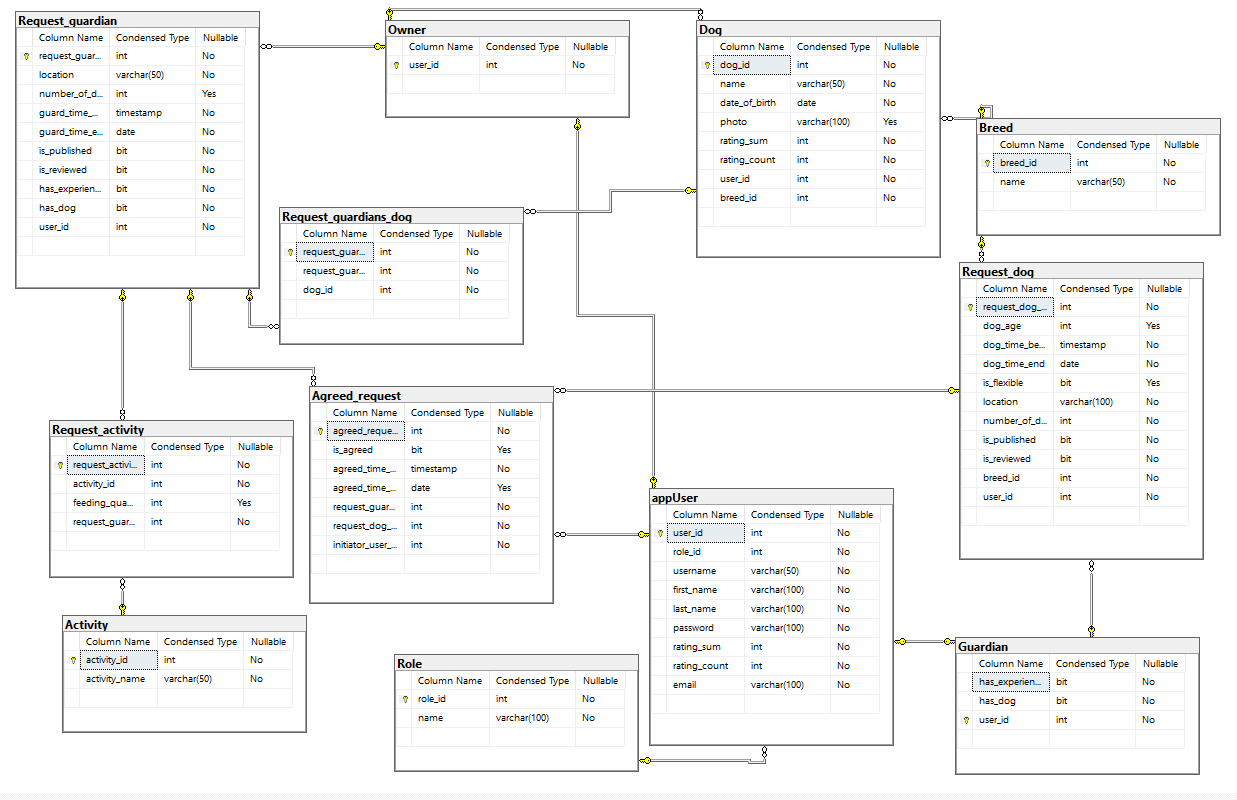
\includegraphics[width=16cm]{slike/dijagramASCP}
				\caption{E-R dijagram baze podataka} 
				\label{fig:E-Rdijagram}
			\end{figure}
			
			\eject
			
			
		\section{Dijagram razreda}
		
			Na slici 4.2 prikazani su razredi koji pripadaju backend dijelu MVC arhitekture.  Zbog lakše organizacije, razredi su podijeljeni logički po pravu pristupa metodama određenih aktora, kako bi se smanjila prenapučenost unutar dijagrama, prikazane su samo ovisnosti između razreda koji pripadaju istom dijelu dijagrama. Iz naziva i tipova atributa u razredima može se zaključiti vrsta ovisnosti među različitim razredima.
			
			\begin{figure}[htb]
				\centering
				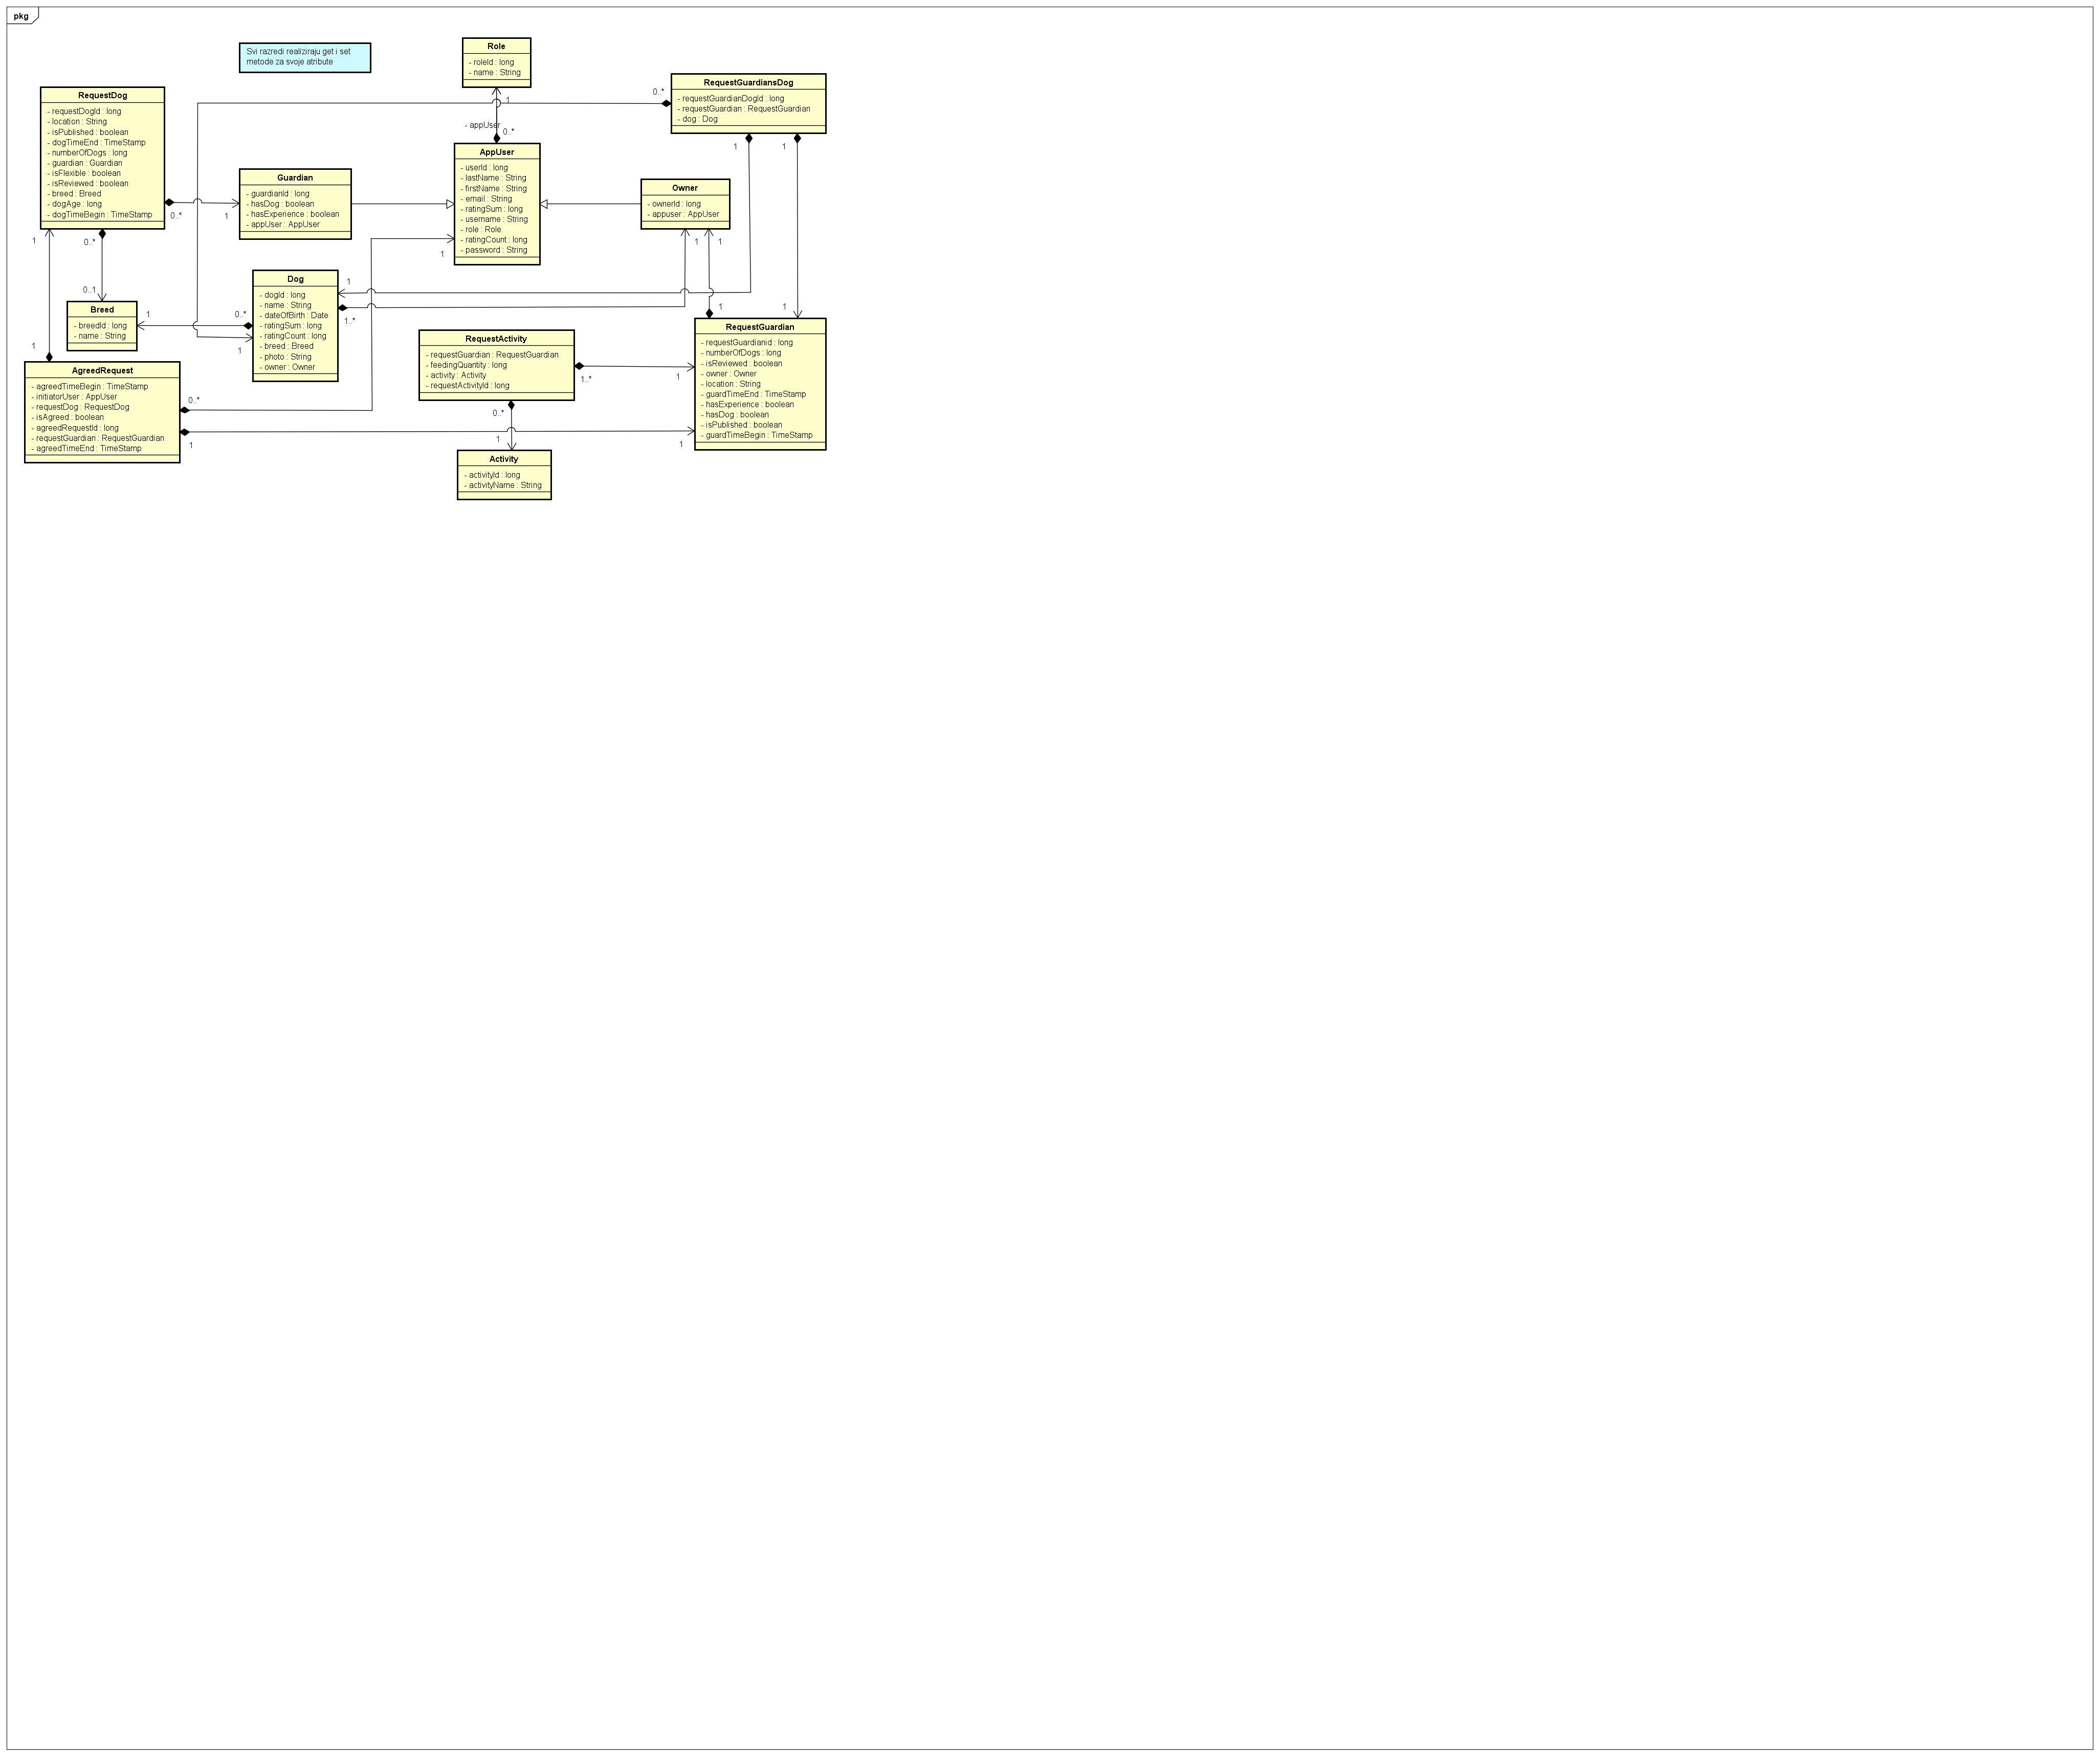
\includegraphics[width=16cm]{slike/Class Diagram}
				\caption{Dijagram razreda - dio Models} 
				\label{fig:Class-Diagram}
			\end{figure}
		
			Model razredi preslikavaju strukturu baze podataka u aplikaciji. Implementirane metode direktno komuniciraju s bazom podataka te vraćaju tražene podatke.\\
			Razred AppUser predstavlja korisnika web aplikacije koji se može registrirati unoseći potrebne informacije. Odabravši pritom ulogu (razred Role), on se priključuje web aplikaciji kao vlasnik pasa (razred Owner) i/ili kao čuvar pasa (razred Guardian). Administrator je korisnik aplikacije koji ima sve mogućnosti App Usera. Vlasnik pasa može dodati vlastitog psa u sustav (razred Dog). Vlasnik i čuvar mogu tražiti čuvara za svog pasa (razred RequestGuardian) odnosno psa za čuvanje (razred RequestDog). Vlasnik može još pregledati ima li čuvar pasa (razred RequestGuardiansDog) i tražiti koju aktivnost će čuvar raditi sa psom (razredi Activity i RequestActivity). Dogovor vlasnika i čuvara predstavlja razred AgreedRequest.
			
			\eject
			
			\textbf{\textit{dio 2. revizije}}\\			
			
			\textit{Prilikom druge predaje projekta dijagram razreda i opisi moraju odgovarati stvarnom stanju implementacije}
			
			
			
			\eject
		
		\section{Dijagram stanja}
			
			
			\textbf{\textit{dio 2. revizije}}\\
			
			\textit{Potrebno je priložiti dijagram stanja i opisati ga. Dovoljan je jedan dijagram stanja koji prikazuje \textbf{značajan dio funkcionalnosti} sustava. Na primjer, stanja korisničkog sučelja i tijek korištenja neke ključne funkcionalnosti jesu značajan dio sustava, a registracija i prijava nisu. }
			
			
			\eject 
		
		\section{Dijagram aktivnosti}
			
			\textbf{\textit{dio 2. revizije}}\\
			
			 \textit{Potrebno je priložiti dijagram aktivnosti s pripadajućim opisom. Dijagram aktivnosti treba prikazivati značajan dio sustava.}
			
			\eject
		\section{Dijagram komponenti}
		
			\textbf{\textit{dio 2. revizije}}\\
		
			 \textit{Potrebno je priložiti dijagram komponenti s pripadajućim opisom. Dijagram komponenti treba prikazivati strukturu cijele aplikacije.}